\documentclass[sigconf]{acmart}

\usepackage{booktabs} % For formal tables
\usepackage{subfig}
\usepackage{amsmath}
\usepackage{listings}
\usepackage{color}
\usepackage[font=small,labelfont=bf]{caption}

\definecolor{dkgreen}{rgb}{0,0.6,0}
\definecolor{gray}{rgb}{0.5,0.5,0.5}
\definecolor{mauve}{rgb}{0.58,0,0.82}

 
\lstset{frame=tb,
  aboveskip=3mm,
  belowskip=3mm,
  showstringspaces=false,
  columns=flexible,
  basicstyle={\footnotesize\ttfamily},
  numbers=none,
  numberstyle=\tiny\color{gray},
  keywordstyle=\color{blue},
  commentstyle=\color{dkgreen},
  stringstyle=\color{mauve},
  breaklines=true,
  breakatwhitespace=true,
  tabsize=3
}


\begin{document}
\title{DataONE RunManager: a \color{dkgreen}{scientific workflow provenance data management tool}}

%\author{Ben Trovato}
%\orcid{1234-5678-9012}
%\affiliation{%
%  \institution{Institute for Clarity in Documentation}
%  \streetaddress{P.O. Box 1212}
%  \city{Dublin} 
%  \state{Ohio} 
%  \postcode{43017-6221}
%}
%\email{trovato@corporation.com}

%\author{G.K.M. Tobin}
%\affiliation{%
%  \institution{Institute for Clarity in Documentation}
%  \streetaddress{P.O. Box 1212}
% \city{Dublin} 
%  \state{Ohio} 
%  \postcode{43017-6221}
%}
%\email{webmaster@marysville-ohio.com}

%\author{Lars Th{\o}rv{\"a}ld}
%\affiliation{%
%  \institution{The Th{\o}rv{\"a}ld Group}
%  \streetaddress{1 Th{\o}rv{\"a}ld Circle}
%  \city{Hekla} 
%  \country{Iceland}}
%\email{larst@affiliation.org}


% The default list of authors is too long for headers}
%\renewcommand{\shortauthors}{B. Trovato et al.}


\begin{abstract}
In this demo, we demonstrate a \textcolor{dkgreen}{scientific workflow provenance data management tool} -- DataONE RunManager that  can capture, store, query, visualize, and publish of a single Matlab script or multiple Matlab script runs. The important features of DataONE RunManager include: (1) There are three forms of data provenance supported by RunManager: prospective provenance, retrospective provenance, and hybrid provenance; (2) \textcolor{dkgreen}{Query-based approach is used for data dependency analysis. For} a workflow project, we have multiple provenance graphs consisting of a graph of prospective provenance, a graph of hybrid provenance, a graph of retrospective multiple\_scripts\_multiple\_runs provenance. 
\end{abstract}


\keywords{prospective provenance, hybrid provenance, retrospective provenance, provenance query}

\maketitle

\section{Introduction}

Provenance plays an important role in \textcolor{dkgreen}{modelling}, designing, debugging, testing, reliability and maintenance~\cite{Ajila:1995, Arnold:1996}. A considerable amount of research has been done on investigating methods of harvesting provenance information from scripts and runs of scripts, ranging from conventional approaches, e.g. research compendium (folder layouts) and logging to recent provenance tools, such as YesWorkflow~\cite{yesworkflow}, noWorkflow~\cite{noworkflow}, RDataTracker~\cite{rdatatracker}, Reprozip~\cite{reprozip}, RunManager~\cite{runmanager}. This demo will illustrate the prospective and retrospective provenance that are captured by YesWorkflow and DataONE RunManagers, and how to query, and visualize using a combination of tools for exposing both prospective, retrospective and hybrid provenance. 

The DataONE RunManager is a \textcolor{dkgreen}{scientific workflow provenance data management tool}. It can capture, store, query, visualize, and publish of one or multiple Matlab or R script runs. \textcolor{dkgreen}{YesWorkflow (YW) is a prospective provenance tool allowing users to model and design prospective provenance via YW tags.} There are three types of provenance demonstrated in our demo: prospective provenance, retrospective provenance, and hybrid provenance. The retrospective provenance captured during a script execution includes information about the script that was run, files that were read or written, and details about the execution environment at the time of execution.

DataONE RunManager provides two implementations: \texttt{recordr} R package and \texttt{matlab-dataone} toolbox. The RunManagers can capture \textcolor{dkgreen}{retrospective} provenance information \textcolor{dkgreen}{when a running of R or Matlab script} and generate a data package. A DataONE package includes scripts, a list of input files, and a list of generated files, science metadata that are associated with the run. In addition, a DataONE data package can be efficiently archived so that the past versions of files can be retrieved for a run in order to investigate previous versions of processing or analysis, support reproducibility, and provide an easy way to publish data products and all files that contributed to those products to a data repository such as the DataONE network.

Then, we show three forms of data provenance. Particularly, we present multi\_scripts\_multi\_runs provenance in DataONE provenance database. From the multi\_scripts\_multi\_runs provenance, it enables a longitudinal view of a typical real-life scientific workflow that consists of multiple phases. Since computational and data science experiments can often last days, weeks, or even months and often require the execution of multiple scripts or workflows with varying input datasets and parameters, some of these script runs appear as chained together implicitly via intermediate data. Multiple\_scripts\_multi\_runs provenance graphs can be joined on file path, file content, etc.

We use query-based approach for provenance analysis. A query is implemented in Prolog and SQL. A graph is used to represent the query results. For a workflow project, we have multiple provenance graphs consisting of a graph of prospective provenance, a graph of hybrid provenance, a graph of retrospective multi-run provenance. 
 
The rest of this paper is organized as follows. The three forms of data provenance used in RunManagers are presented in Section~\ref{architecture-prov-query}. Section~\ref{usecases} discusses two example use cases whereas Section~\ref{conclusions} concludes the paper.

\paragraph{\textit{\bf Related Work}}
Table~\ref{tab:prov_tools} presents a representative set of related provenance tools for provenance collection. YesWorkflow provides prospective graph revealing the data dependencies at the conceptual workflow level. URI-template specifies a file path pattern while user-defined log-files capture runtime provenance observables at any level of granularity. The noWorkflow system (NW)\cite{noworkflow} captures code-level retrospective provenance by employing a Python profiling library to obtain Python function call chains and variable assignments. The DataONE RunManagers\cite{runmanager} overload and thus intercept file I/O operations to automatically capture runtime observables at the file level. 

\begin{table*}
\caption{Various Provenance Tools and Methods Breakdown}
\label{tab:prov_tools}
\footnotesize
\begin{tabular}{llll}
  \toprule
                          & \begin{tabular}{@{}l@{}}Language: Application / \\ Implementation\end{tabular}     & Scope & Methods \\
 \midrule
  YesWorkflow   & Any / Java  & \begin{tabular}{@{}l@{}}Prospective \\ Provenance\end{tabular} & \begin{tabular}{@{}l@{}}Annotations added by users;  \\ language independent \end{tabular}\\
 \hline
  URI-templates & Any / Any &   \begin{tabular}{@{}l@{}}Retrospective \\ Provenance\end{tabular} & \begin{tabular}{@{}l@{}}Templates matching with runtime \\ file locations; language independent\end{tabular}  \\
  \hline
  User-de�ned log-�les  & Any / Any  & \begin{tabular}{@{}l@{}}User-defined \\ Retrospective \\Provenance \end{tabular}   &   \begin{tabular}{@{}l@{}}Exported runtime variables and \\ files provenance by users\end{tabular}   \\
  \hline
  noWorkflow     & Python / Python & \begin{tabular}{@{}l@{}}Retrospective \\ Provenance\end{tabular}  & \begin{tabular}{@{}l@{}}Runtime function calls, variables, \\ file inputs/outputs, \\ execution environmental information\end{tabular}  \\
  \hline
  RunManagers    & \begin{tabular}{@{}l@{}}R / R \\ MATLAB / MATLAB\end{tabular} & \begin{tabular}{@{}l@{}}Retrospective \\ Provenance\end{tabular}  & \begin{tabular}{@{}l@{}}Runtime file inputs/outputs, \\ execution environmental information\end{tabular} \\
  \bottomrule
\end{tabular}
\end{table*}

\section{Three forms provenance}  \label{architecture-prov-query}

\texttt{Data provenance} is metadata that describes the origin and processing history of a data artifact. In the computational and data sciences, we can distinguish three forms of data provenance, i.e., \texttt{prospective provenance}, \texttt{retrospective provenance}, and \texttt{hybrid provenance}. The prospective provenance describes the general workflow by which data is produced, while the retrospective provenance consists of runtime observables, e.g., read and generated files during a script run (coarse-grained observables). Fine-grained provenance can be captured as well, e.g., changes to individual data records, program variables, parameter settings, etc. \texttt{Hybrid provenance} can be defined as a graph containing an alternation of process steps, situated in the context of the prospective workflow graph, and of the specific instances of data elements that have been generated and consumed by executions of those steps. The data elements can be instantiated to document the specific files used in a concrete workflow run. 

\begin{lstlisting} [caption={YW annotation block in C3C4 Matlab script},label={fig:yw_matlab_tags}, language=Matlab] 
%% Load input: long-term monthly mean precipitation data
% @BEGIN fetch_monthly_mean_precipitation_data
% @in mean_precip @URI 
% file:inputs/narr_apcp_rescaled_monthly/
% apcp_monthly_{start_year}_{end_year}_mean.{month}.nc
% @out Rain @AS Rain_Matrix
Rain=zeros(ncols,nrows,12);
for m=1:12
   rncid=netcdf.open(strcat(
    'inputs/narr_apcp_rescaled_monthly/monthly_2000_2010_mean.',
    num2str(m),'.nc'), 'NC_NOWRITE');
   rvid=netcdf.inqVarID(rncid, 'apcp_monthly_mean');
   Rain(:,:,m)=netcdf.getVar(rncid,rvid);
   netcdf.close(rncid)
end
% @END fetch_monthly_mean_precipitation_data
\end{lstlisting}

YesWorkflow (YW) is a prospective provenance tool allowing users to easily recover high-level workflow models latent in scripts using simple user-annotations embedded as script comments\cite{yesworkflow}. List~\ref{fig:yw_matlab_tags} shows a code snippet from a MATLAB script with YW annotations. The @begin and @end tags are used to mark code blocks (i.e., processing steps in the YW model); @in and @out tags are used to define the dataflow between blocks; the @uri template (which is paired with an @in tag) is used to define a where the data file is located. Note that @uri templates define a metadata pattern via so-called template variables (here: ${start\_year}$, ${end\_year}$, and ${month}$). In this way, the script author can document the folder structure and file-naming conventions used by the script. List~\ref{fig:yw_R_tags} shows a YW annotation block \textcolor{dkgreen}{modelling a dataflow for \texttt{lsp\_status\_file} } in a R script \textcolor{dkgreen}{as shown in} Figure~\ref{fig:hs_yw}. \textcolor{dkgreen}{The optional @param tag is used to specify the input and output parameters.} 

%-------------------------------------------------------------
\begin{lstlisting} [caption={YW annotation block in one OHIBC R script},label={fig:yw_R_tags}, language=R] 
# @BEGIN output_estimate_status_file_by_region_since_1980
# @param year_span
# @param dir_goal
# @in area_protected_total_file @URI file:{dir_goal}/output/area_protected_total.csv
# @in status_file_handle
# @out status_df_data
status_df <- read.csv(file.path(dir_goal, 'output', 'area_protected_total.csv')) %>%
  select(rgn_id, year, lsp_status) %>%
  filter(year > max(year) - year_span)
# @END output_estimate_status_file_by_region_since_1980  
  
# @BEGIN write_status_to_csv_file
# @in status_df_data
# @out lsp_status_file @URI file:{dir_goal}/output/lsp_status.csv
write.csv(status_df, status_file)
# @END write_status_to_csv_file 
\end{lstlisting}


A scientific workflow script can run inside of RunManager by invoking the \texttt{record} function. The RunManager can automatically capture \textcolor{dkgreen}{file-level} retrospective provenance \textcolor{dkgreen}{by overloading and thus intercepting} file I/O operations. \textcolor{dkgreen}{The automated approach is efficient and useful for scientists.} RunManagers support the following APIs: \texttt{record},  \texttt{startRecord}, \texttt{endRecord}, \texttt{listRuns}, \texttt{deleteRuns}, \texttt{viewRun(s)}, \texttt{traceRuns} for R, \texttt{plotRuns} for R and \texttt{publishRun} in order to capture, search, archive, visualize, and publish a script run. \textcolor{dkgreen}{Then, the captured provenance information is saved to local database}. \textcolor{dkgreen}{The database tables include:} \texttt{execution metadata}, \texttt{file metadata}, \texttt{tag}, \texttt{module dependencies} for MATLAB and \texttt{provenance relationships} for R. \textcolor{dkgreen}{In addition, the provenance database} can be exported as \textcolor{dkgreen}{Prolog} facts. Retrospective provenance graphs can be rendered from the exported \textcolor{dkgreen}{Prolog} facts. \textcolor{dkgreen}{With YesWorkflow and RunManager, scientists can model, design, execute, debug, re-configure and re-run their analysis and visualization pipelines. Provenance is useful for a scientist to interpret their workflow results and for other scientists to establish trust in the experimental result~\cite{Barga2008}.}

For example, a multi\_scripts\_multi\_runs provenance sub-graph can be produced by executing a Prolog query \footnote{\label{query1}\url{https://github.com/yesworkflow-org/yw-idcc-17/blob/master/OHIBC\_Howe\_Sound\_project/multi\_runs\_retrospective\_provenance\_queries/queries/render\_rm\_graph\_upstream\_of\_file\_q1\_sha256.sh}} which consists of four Prolog queries using the exported \textcolor{dkgreen}{Prolog} facts. A example set of logical rules are highlighted in List~\ref{logic_rule_multi_prov}. The joining operation is based on file content (hash code). For the recursive rules \texttt{rm\_file\_downstream} computes all upstream files for the given file \texttt{Sha256\_2}. It has two base cases: one is the file object is itself downstream file object and the other is immediate derived relationship.  

\begin{lstlisting}  [caption={Prolog rules for multiple scripts multiple runs provenance},label={logic_rule_multi_prov}, language=bash] 
:- table rm_file_immediately_downstream/2.
rm_file_immediately_downstream(Sha256_1, Sha256_2) :-
    exec_used_files(_, E, _, _, _, Sha256_1, _, _, _),
    exec_generated_files(_, E, _, _, _, Sha256_2, _, _, _).

# Base case 1.
:- table rm_file_downstream/2.
rm_file_downstream(Sha256_1, Sha256_2) :-
    Sha256_1 = Sha256_2.
# Base case 2.    
rm_file_downstream(Sha256_1, Sha256_2) :-
    rm_file_immediately_downstream(Sha256_1, Sha256_2).   
# Recursive part.
rm_file_downstream(Sha256_1, Sha256_2):-
    rm_file_immediately_downstream(Sha256_1, S),
    rm_file_downstream(S, Sha256_2).

# The rule gv_nodes__files__upstream_of_file_sha256 computes all file objects which has a given hashcode (DataSha256).
gv_nodes__files__upstream_of_file_sha256(_, DataSha256) :-
    rm_file_downstream(Sha256, DataSha256),
    filemeta(_,_,FilePath,Sha256,_,_,_,_,_,_,_),
    gv_labeled_node_sha256(Sha256, FilePath),
    fail
    ;
    true.
# The rule gv_edges__execution_to_file__upstream_of_file_sha256 draws edges from an execution object to file objects by first finding all upstream file objects for a given hashcode (DownstreamDataSha256).          
gv_edges__execution_to_file__upstream_of_file_sha256(_, DownstreamDataSha256) :-
    rm_file_downstream(DataSha256, DownstreamDataSha256),
    exec_generated_files(_,ExecutionId,_,_,_,DataSha256,_,_,_),
    gv_unlabeled_edge_sha256(ExecutionId, DataSha256),
    fail
    ;
    true.
\end{lstlisting}  

Hybrid provenance can be derived using logic rules. The approach of creating hybrid provenance is as follows: after a script run is completed, the retrospective provenance information are collected and populated to Sqlite provenance database. Then, Matlab RunManager has a function to export content of tables \texttt{filemeta} as a list of input and output file paths that are fed to \texttt{yw-matlab bridge}. The bridge will match the URI templates with the exported file list and the logical rule for producing hybrid provenance is shown in List~\ref{logic_rule_hybrid_prov}.

\begin{lstlisting}  [caption={Prolog rules for computing hybrid provenance},label={logic_rule_hybrid_prov}, language=bash] 
:- table data_uri_resource/2. 
data_uri_resource(DataId, ResourceURI) :- 
     data_resource(DataId,ResourceId), 
     resource(ResourceId, ResourceURI). 
\end{lstlisting}  

After \textcolor{dkgreen}{obtaining} three forms of \textcolor{dkgreen}{data provenance}, we can demonstrate the provenance dependency with \textcolor{dkgreen}{queries}. We have developed both SQL queries and  Prolog rule-based queries (e.g., List~\ref{logic_rule_multi_prov} and ~\ref{logic_rule_hybrid_prov}) against \textcolor{dkgreen}{three forms of provenance}. For example: What outputs does the workflow (script) have? Advanced provenance queries can take the form of regular path queries (RPQs), tree-structure queries, or graph queries and show the data lineage hidden in the provenance information. For example: (1) What are the ancestors or descendants of a given output in a prospective provenance graph? (2) What are the ancestors or descendants of a given output in a retrospective- or hybrid- provenance graph? (3) Which possible execution (i.e., dataflow) paths satisfy a given regular path expression? The queries and results are demonstrated \textcolor{dkgreen}{with two use cases} in Section~\ref{usecases}.


\section{Example Use Cases} \label{usecases}

In this demo, two real-life scientific examples are used: (A) a workflow for Ocean Health Index (OHI) for Howe Sound, British Columbia\cite{ohibc}; (B) a workflow for Carbon3/Carbon4 (C3/C4) soil mapping for North America\cite{MsTMIP-model-driver-data-set, MsTMIP-model-output-data-set}. The OHIBC example calculates the region's status based upon percent of protected area within 1 km inland buffer and percent of protected area within 3 nautical mile offshore buffer, compared to a reference point of 30\% protected area. The data sources used in the OHIBC workflow include: (1) BC-specific WDPA dataset that was created from WDPA global dataset, then rasterize to BC Albers at 500m resolution; (2) BC Parks, Ecological Reserves, and Protected Areas (PEP) data. The OHIBC workflow creates two outputs: one file is for estimate of status by region since 1980 (\texttt{lsp\_status.csv}) and the other file is for estimate of trend by region since 1980 (\texttt{lsp\_trend.csv}). The OHIBC Howe Sound workflow runs in a batch mode.

RunManager can show the prospective provenance and retrospective provenance as graphs for one script. There are eleven R scripts in the OHIBC example.  A user can add YW tags to these R scripts to show prospective provenance graphs. Then, the user can start to run the OHIBC example using RunManager. After the run was done, the retrospective provenances (e.g., the execution of each script, used files, generated files including file path, file content, size, and archived file path) are captured and stored in the database. After exporting retrospective provenance as a list of input and output file paths, hybrid provenance can be derived by joining retrospective provenance and prospective provenance facts using shared resource ids. Figure~\ref{fig:hs_yw} depicts the prospective and hybrid graphs. 

\begin{figure}
  \centering
  \subfloat[prospective provenance graph]{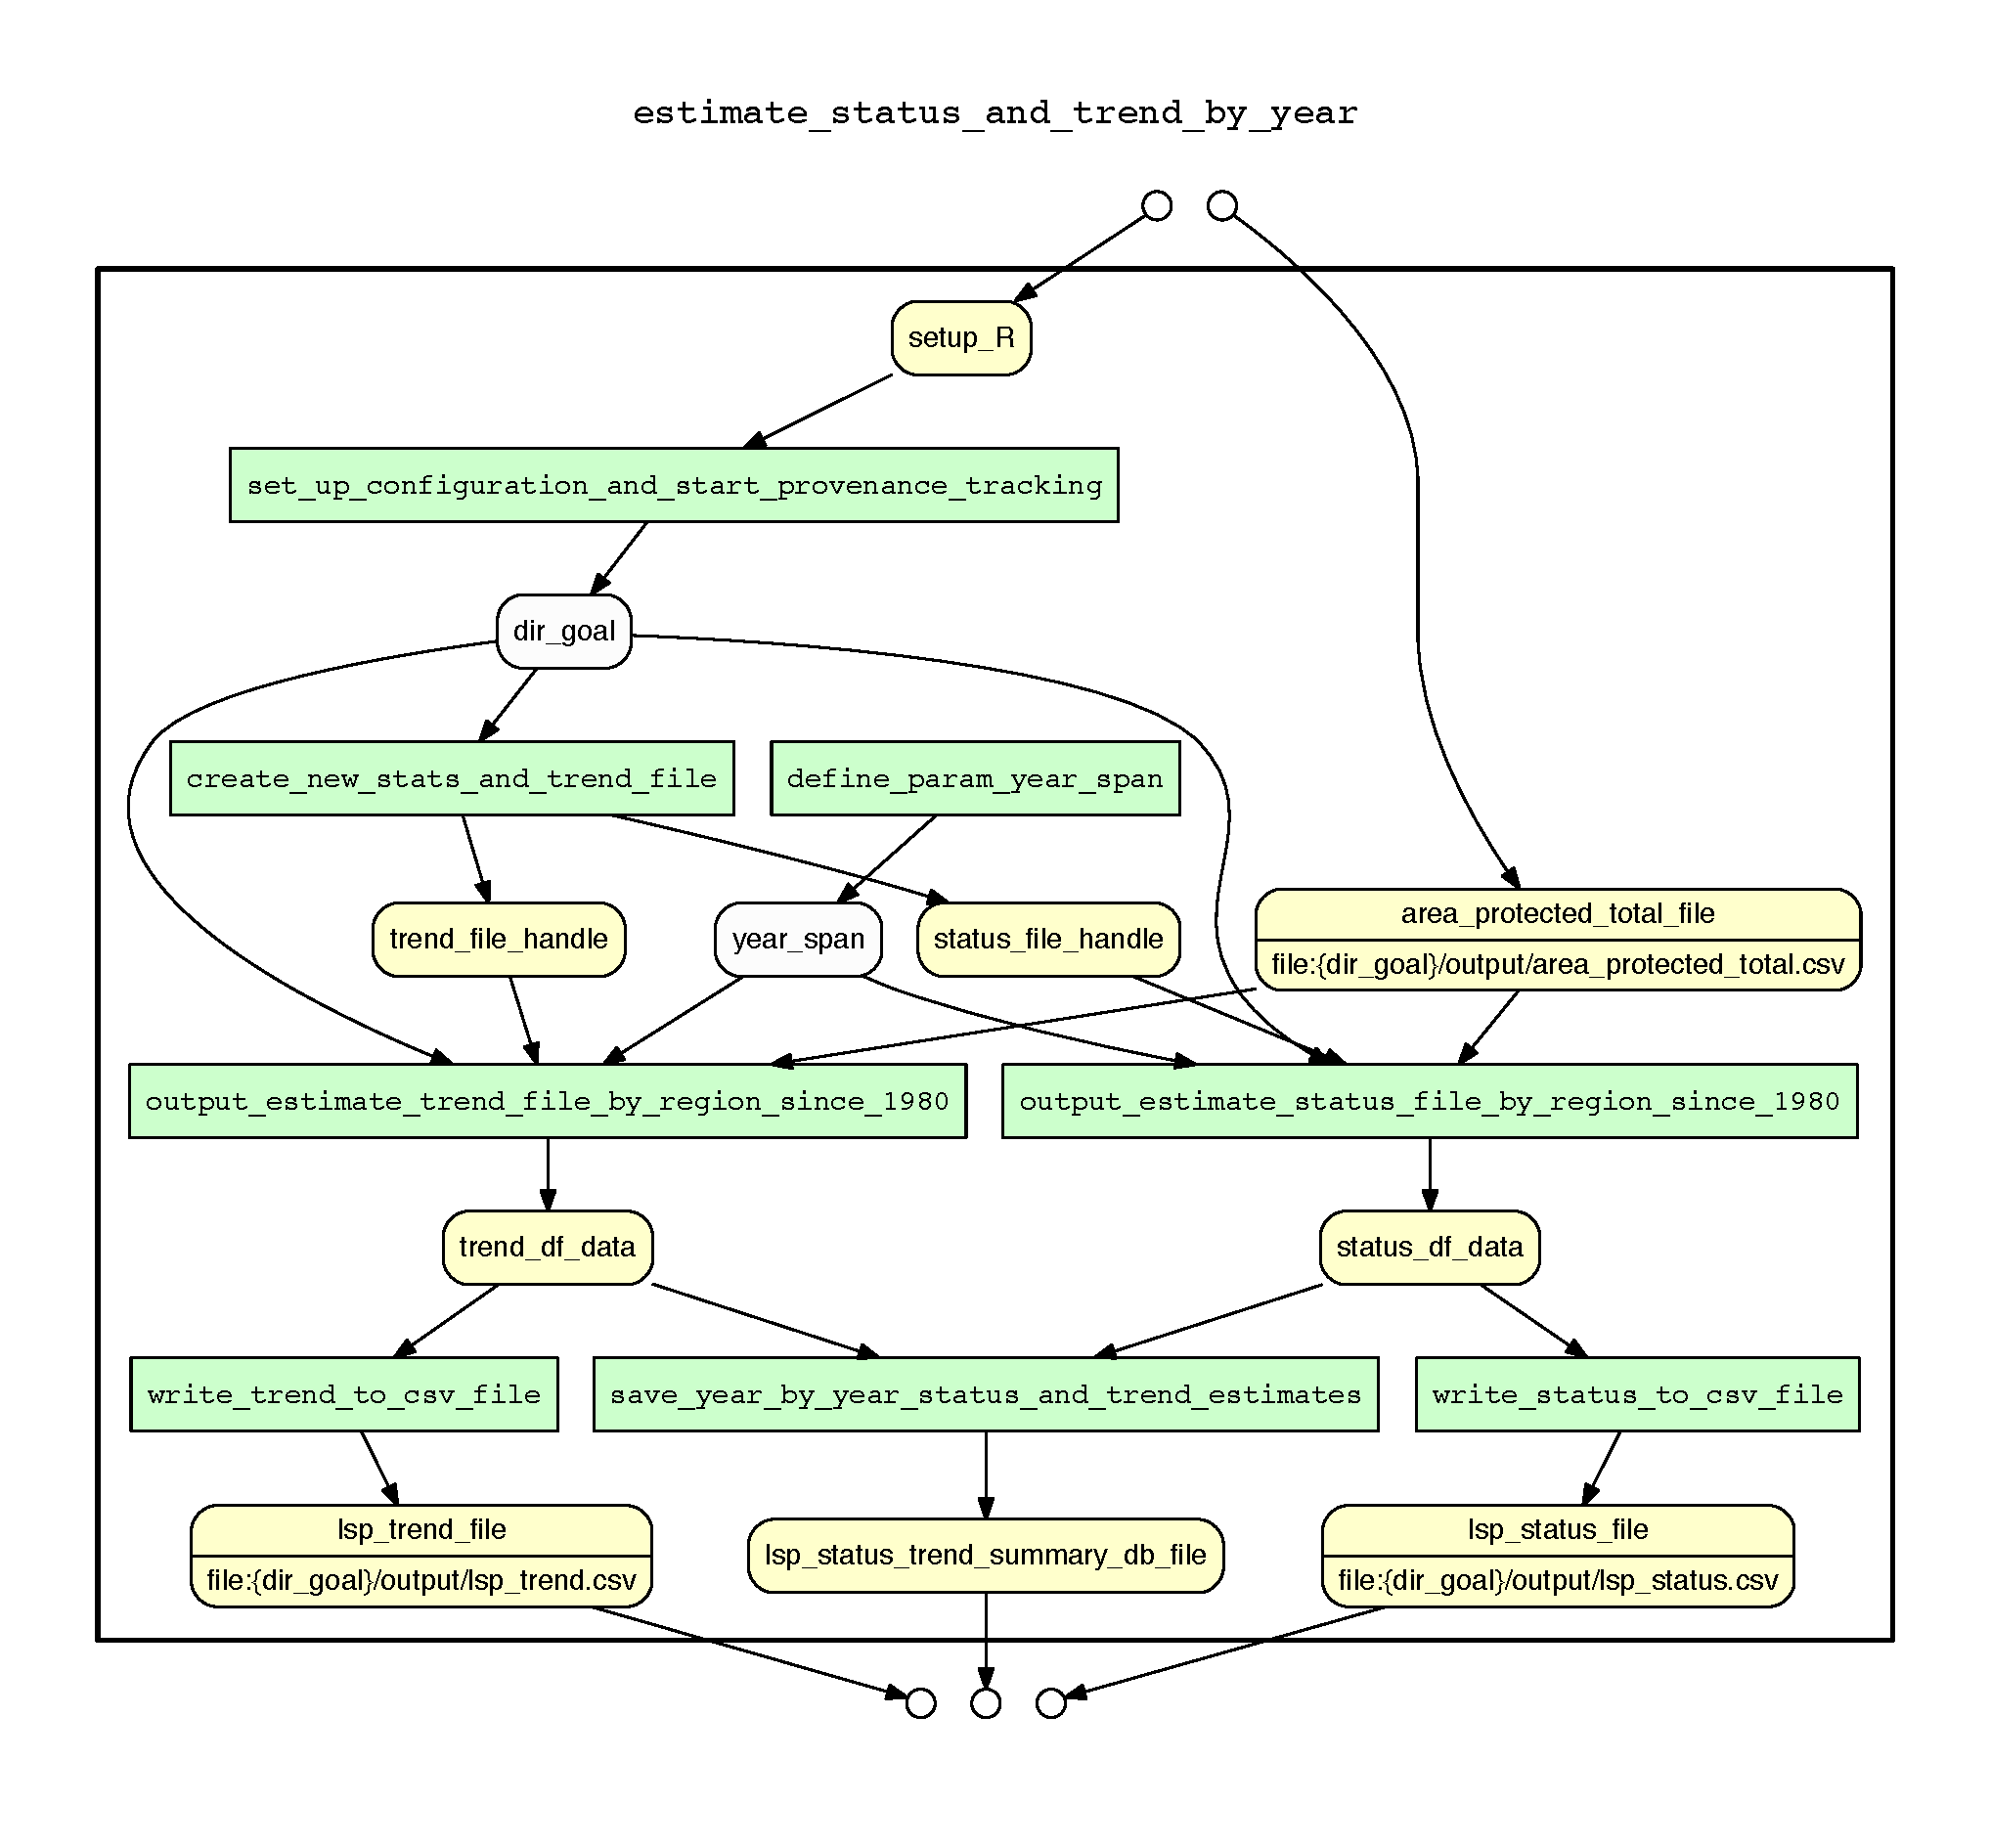
\includegraphics[width=\columnwidth, height=3.3in]{figures/estimate_status_and_trend_by_year_complete_wf_graph_uri}} \\
  \subfloat[hybrid provenance graph]{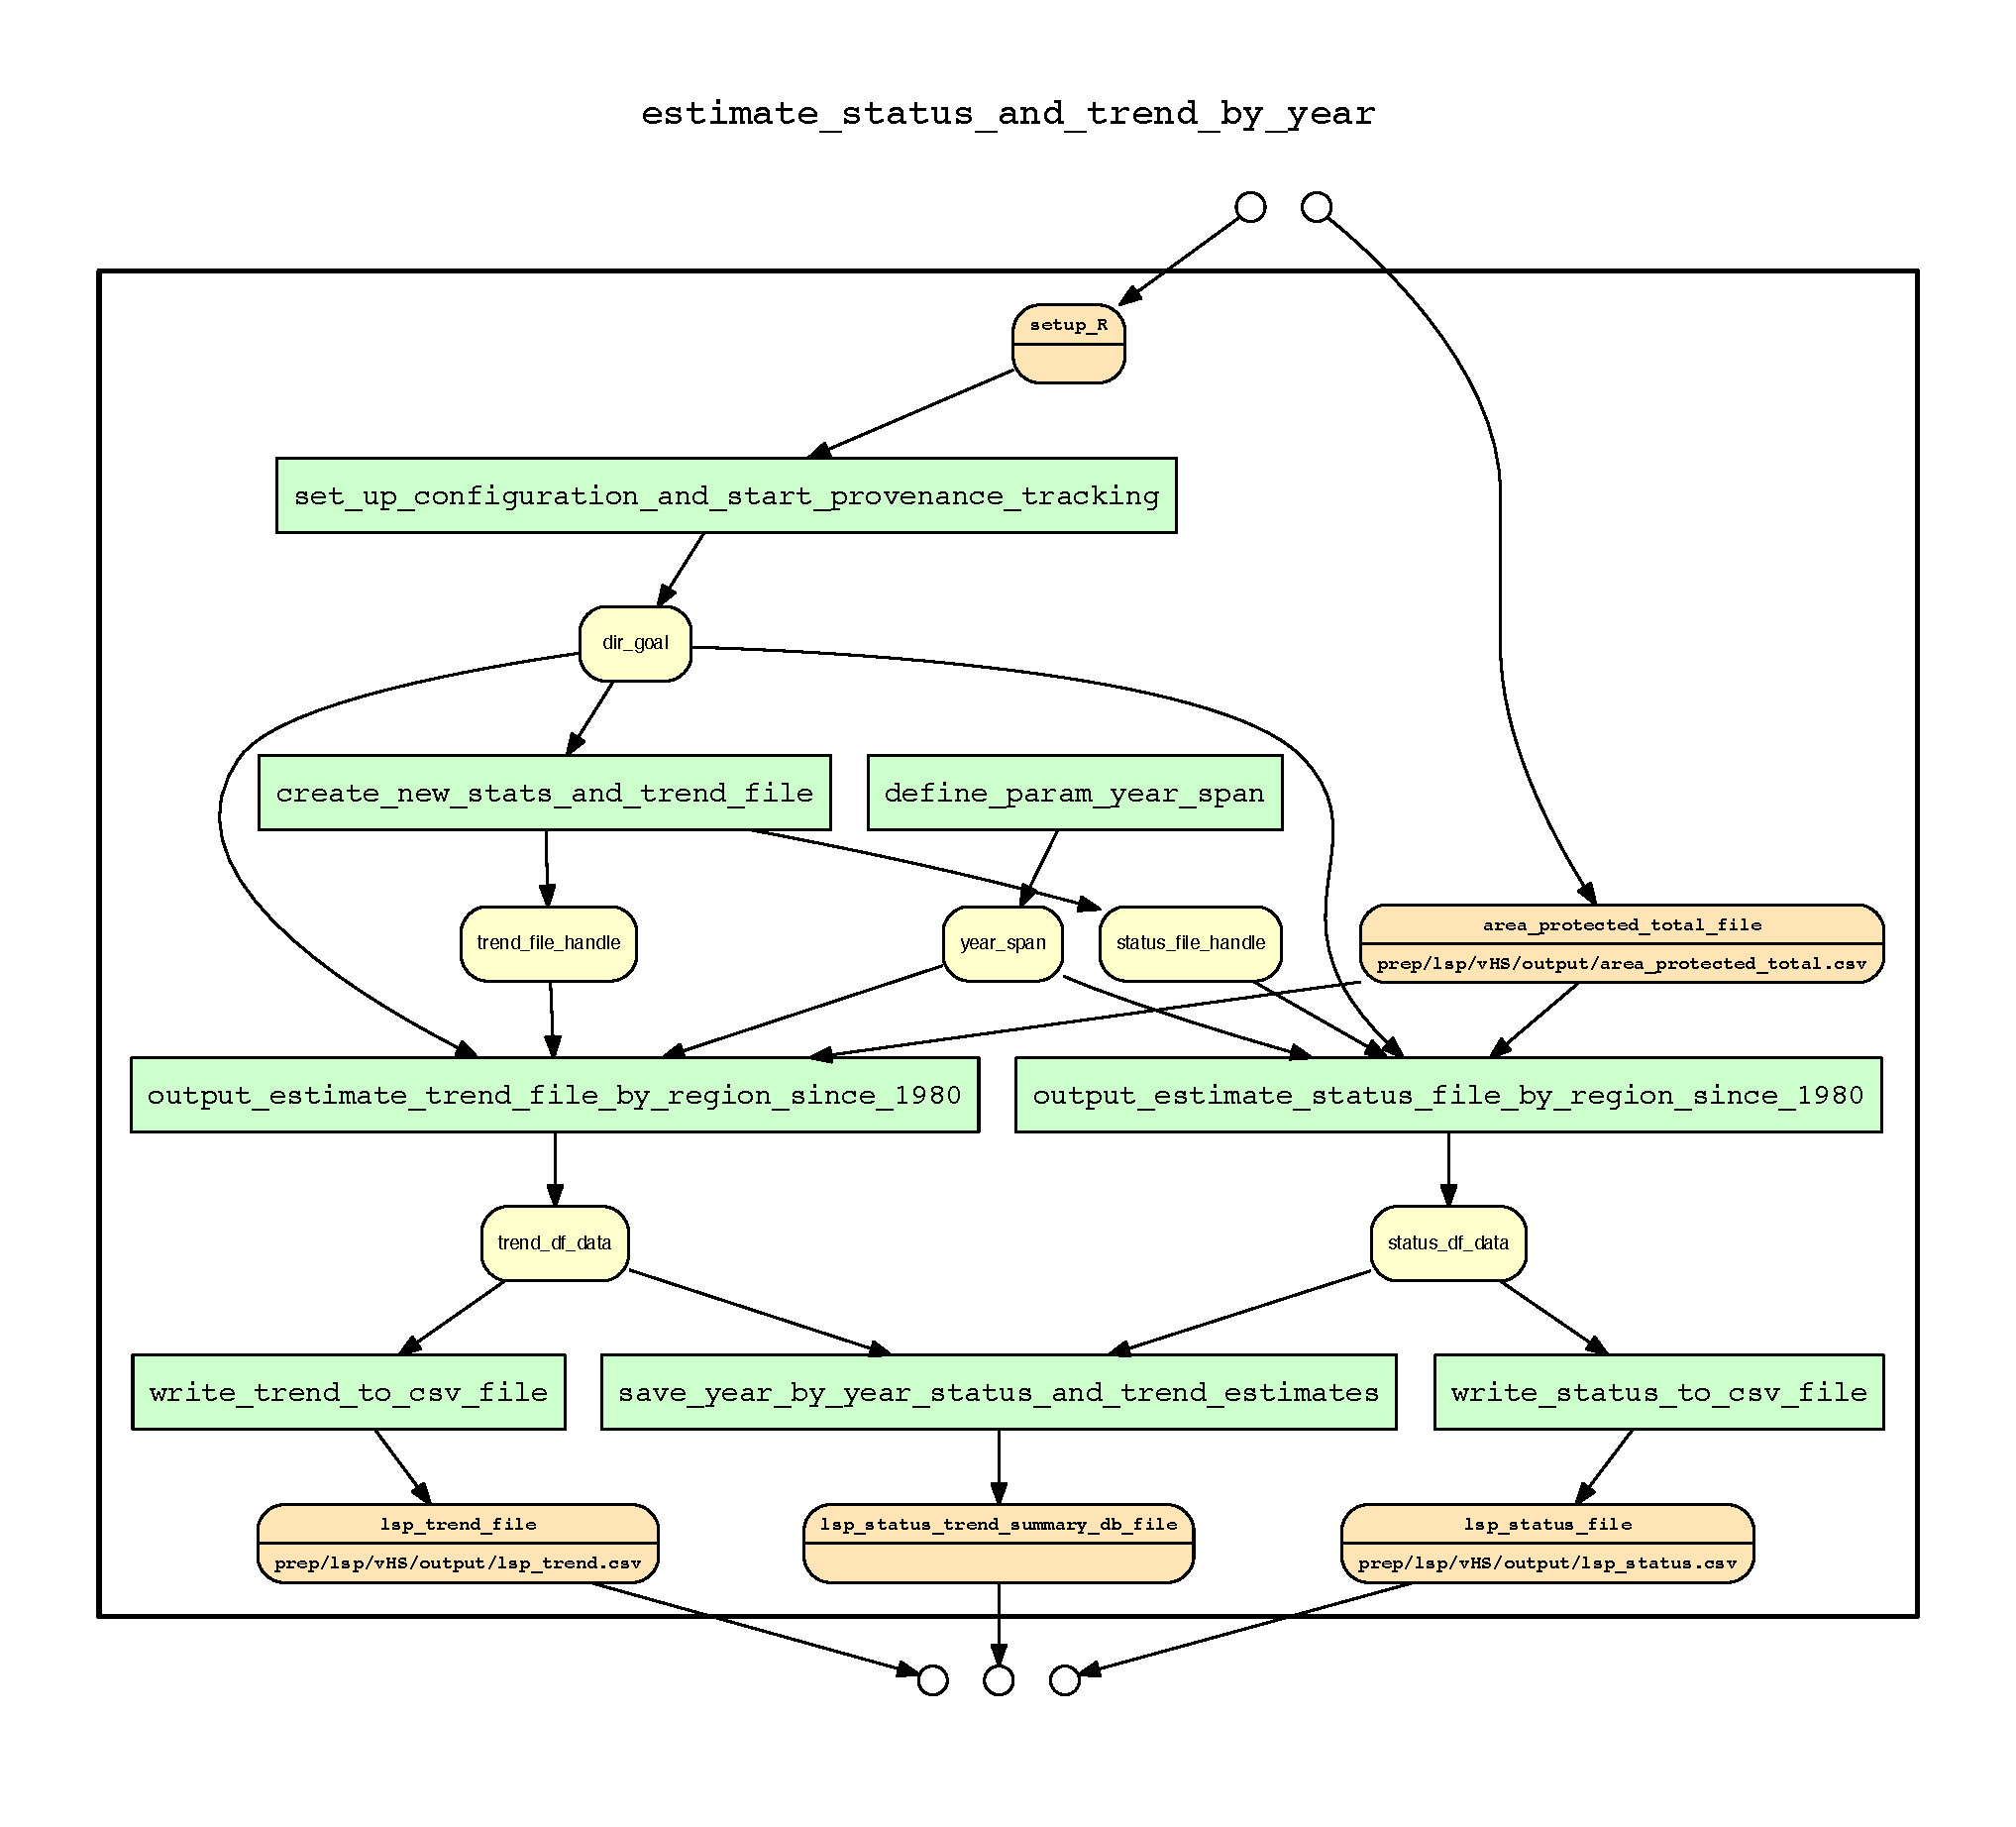
\includegraphics[width=\columnwidth, height=3.3in]{figures/wf_recon_complete_graph_all_observables}}
  \caption{Complete YW prospective and hybrid provenance graphs for the last step script \texttt{estimate\_status\_and\_trend\_by\_year.R}. The green box represents a computation step; a round yellow square box represents a data element declared in the script via YW tags; an orange box represents a data element which URI is expanded with the runtime file path.}
  \label{fig:hs_yw}
\end{figure}


RunManager can review the overview graph for all script runs because RunManager have recorded the execution history for the OHIBC example. Hence, using R RunManager provenance database, the plotRun() API gives us an overview for the OHIBC Howe Sound workflow example shown in Figure~\ref{fig:hs_trace_graph}. Alternatively, using exported Prolog facts from the provenance database, we can use prolog queries to render a complete multi\_scripts\_multi\_runs graph. With exported Prolog facts, we can use query\_based approach to do provenance dependency analysis which will be explained in the next section.

\begin{figure}
  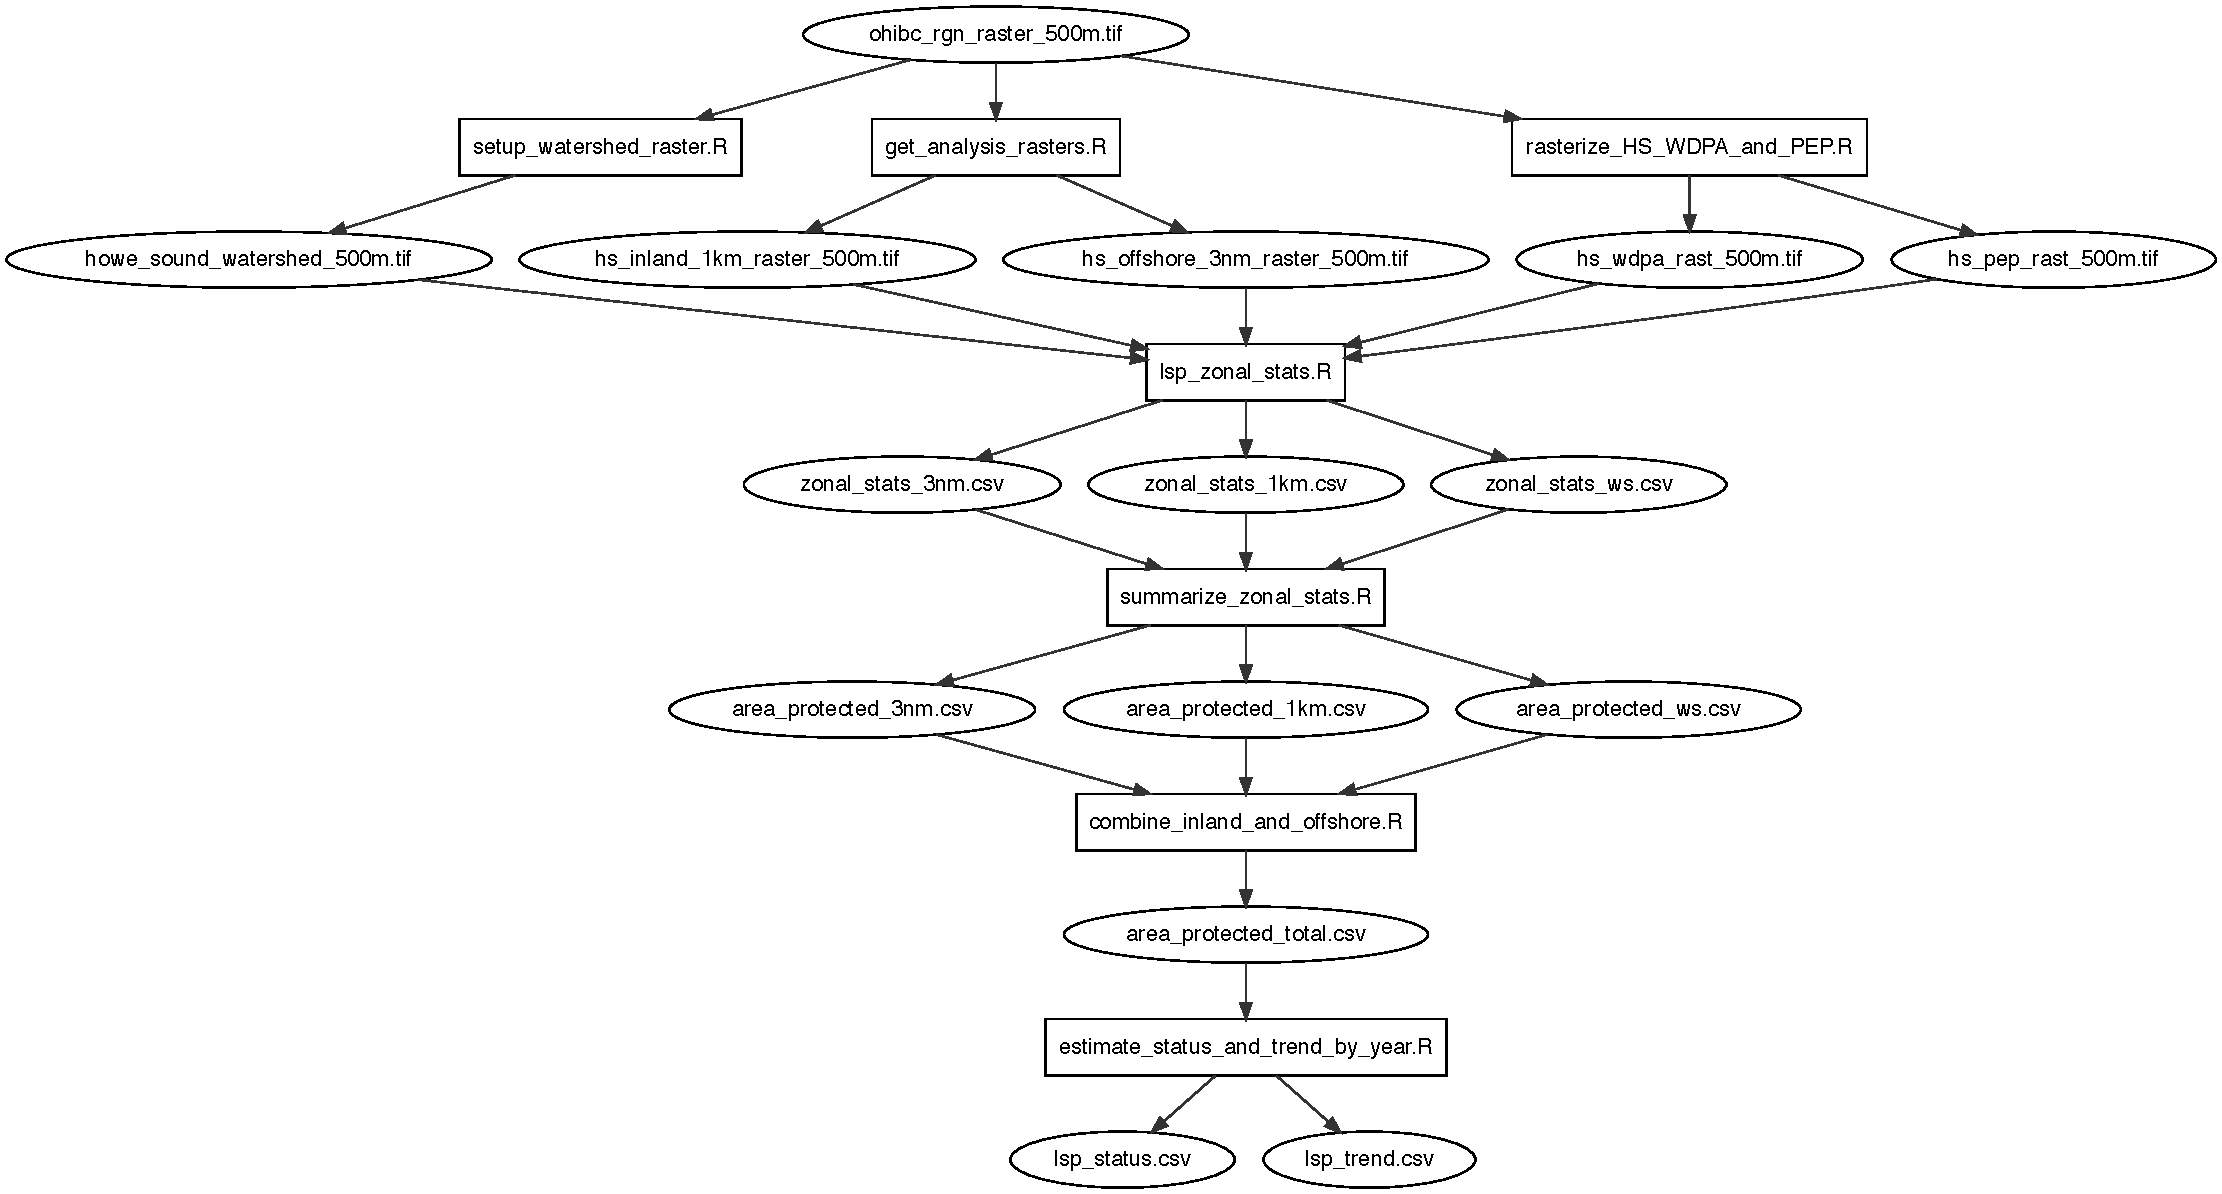
\includegraphics[width=0.9\columnwidth]{figures/trace}
  \caption{Complete retrospective provenance graph for the OHI Howe Sound workflow example plotted by the API \texttt{plotRun()} in DataONE R RunManager}
  \label{fig:hs_trace_graph}
\end{figure}

\paragraph{\textit{\bf Provenance Query Examples}}

The first category provenance query is \texttt{prospective provenance queries} can tell us if an output depends a particular input or if an output depends on all of inputs, see the script \texttt{estimate\_status\_and\_trend\_by\_year.R} in Figure~\ref{fig:hs_yw}). 

The second category provenance query is \texttt{hybrid provenance query}. In a hybrid provenance graph, the ``workflow backbone" is given by the user-declared YW model (prospective provenance) and the execution details are filled in from one or more sources of runtime observables (retrospective provenance). Figure~\ref{fig:hs_yw} shows a hybrid provenance graph for the last script in the OHIBC example \texttt{estimate\_status\_and\_trend\_by\_year.R}. We can see that the yellow round box changes to orange round box and the file path pattern embedded is expanded with runtime relative file paths. Please visit the web link for prospective and hybrid provenance queries \footnote{\label{prov-hybrid-query}\url{https://github.com/yesworkflow-org/yw-idcc-17/tree/master/OHIBC\_Howe\_Sound\_project/hybrid\_provenance\_queries/queries}}. 

The third category provenance query is \texttt{multi\_scripts\_multi\_runs provenance query}. RunManager retrospective provenance queries refer to the runtime retrospective provenance obtained from executing multiple scripts, using RunManager. Since the scripts in a project are usually logically connected through sharing some of their inputs and outputs, the corresponding provenance traces are also connected through shared files. Figure~\ref{fig:hs_trace_graph} shows one complete graph for the OHIBC workflow example using the R provenance relational database and Figure~\ref{fig:upstream_ohibc} shows a upstream retrospective provenance subgraph that is relevant to ``\texttt{lsp\_trend.csv}" output using exported facts. The \texttt{multi\_scripts\_multi\_runs} query can be found at \footnote{\label{multi-runs-query}\url{https://github.com/yesworkflow-org/yw-idcc-17/tree/master/OHIBC\_Howe\_Sound\_project/multi\_runs\_retrospective\_provenance\_queries/queries}}. 

\begin{figure}
  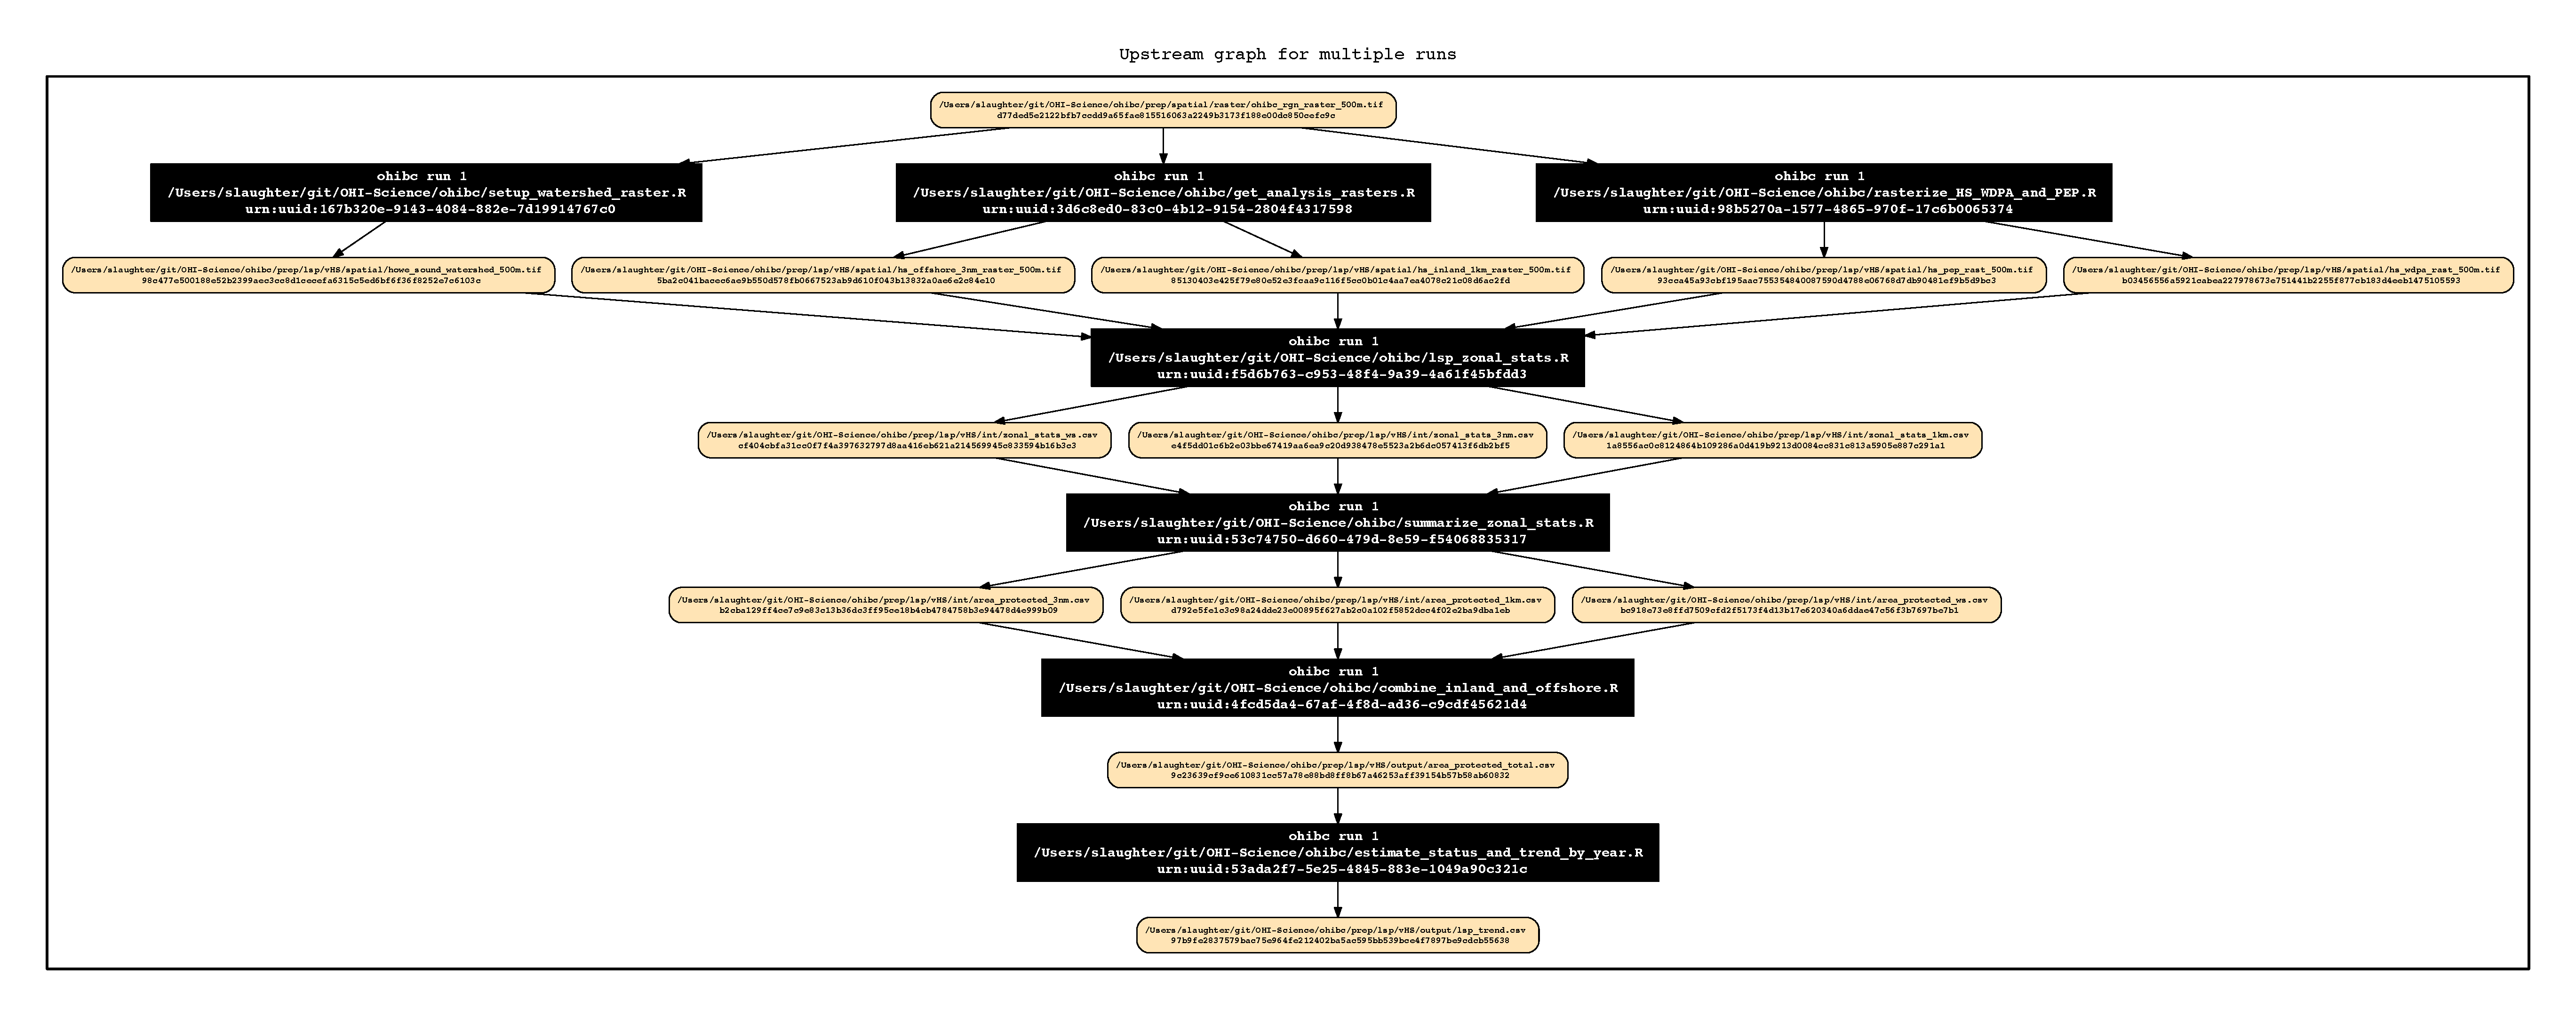
\includegraphics[height=2in,width=\columnwidth, height=3.5in]{figures/OHI_upstream_of_lsp_trend_sha256}
  \caption{Upstream subgraph that is relevant to ``lsp\_trend.csv" output for multi\_scripts\_multi\_runs retrospective provenance for the OHIBC Howe Sound example }
  \label{fig:upstream_ohibc}
\end{figure}

The second example script (in MATLAB) produces Carbon 3/Carbon 4 (C3/C4) soil maps for North America using average rain and air temperature monthly data from year 2000 to 2010. There are two versions for C3C4 example. In the version 1, there is one C3C4 example. The captured provenance and query results for C3C4 version is available at \footnote{\label{C3C4-v1}\url{https://github.com/yesworkflow-org/yw-idcc-17/tree/master/examples/C3C4/results}}. In order to simulate real-life workflow, we create a version 2 C3/C4 example by splitting one script to three phases: \texttt{preparing\_step}, \texttt{examining\_pixels\_for\_grass} and \texttt{generating\_final\_results}. After \texttt{preparing\_step}, a user can run the second script \texttt{examine\_pixels\_for\_grass} for multiple times with different parameters, then writes to the output files in \texttt{generating\_final\_results}. We present such retrospective provenance graphs based on file content (hash code) in Figure~\ref{fig:c3c4v2_filepath} which records a holistic run of the three scripts and the second script was run with two different parameter values (i.e., 2.5 and 5) twice. From Figure~\ref{fig:c3c4v2_filepath}, we find that the second script that ran twice produced two versions of files at the same file location.


\paragraph{\textit{\bf Reproducibility}}

DataONE allows to make experiments reproducible \textcolor{dkgreen}{in three ways}. First, DataONE RunManagers capture both prospective and retrospective provenance \textcolor{dkgreen}{and store related provenance and metadata to database.} \textcolor{dkgreen}{RunManager database enables users to retrieval past version of used and generated data to support reproducibility.} Second, DataONE data repository allows users to package workflow results in a structured DataONE data package and publish to a member node inside a DataONE federation network so that the workflow results (including scripts, data, provenance relationship, science metadata, etc.) can be displayed on DataONE data repository and be shared or linked with other scientific experiments in a larger scale. DataONE package contains provenance information (\texttt{prov:used}, \texttt{prov:wasGeneratedBy}, or \texttt{prov:wasDerivedFrom}) to describe the relationships between digital objects and data packages for reproducibility, instead of only encapsulating digital objects. \textcolor{dkgreen}{Third, the query ability provided by RunManager allows users to reproduce and verify their scientific experiments as graphs without running the scripts after exepriments.}

\section{Conclusions}  \label{conclusions}

Provenance is a useful component of the software development cycle, either to benefit researcher themselves or documenting and sharing code for use by future investigators. For the researcher, the quality of data produced by script runs can be assessed by identifying source data and verifying their quality. With our DataONE RunManager demo, we showcase how RunManager can capture, store, query, visualize, and publish prospective, retrospective and hybrid provenance. \textcolor{dkgreen}{Also, we demonstrate how YesWorkflow can model a scientific script.} Moreover, we demonstrated that provenance queries across heterogeneous provenance sources can yield a more complete and comprehensible picture of data provenance. We also think provenance describing datasets can facilitate data discovery for others. 

%Many provenance tools have been developed to capture, store, query and visualize the provenance produced by scripts and runs of scripts. But there is not enough investigation on what kind of provenance queries can be answered from the provenance information at prospective and retrospective provenance levels. Our research on prospective, hybrid and retrospective provenance queries allow researchers to use simple queries and a subset of advanced queries to query across YW model and various retrospective provenance sources to produce interesting provenance artifacts. 
      
\bibliographystyle{ACM-Reference-Format}
\bibliography{sigproc} 

\appendix
\section{Example retrospective provenance subgraph}

\begin{figure}
  \centering
  %\subfloat[label1]{{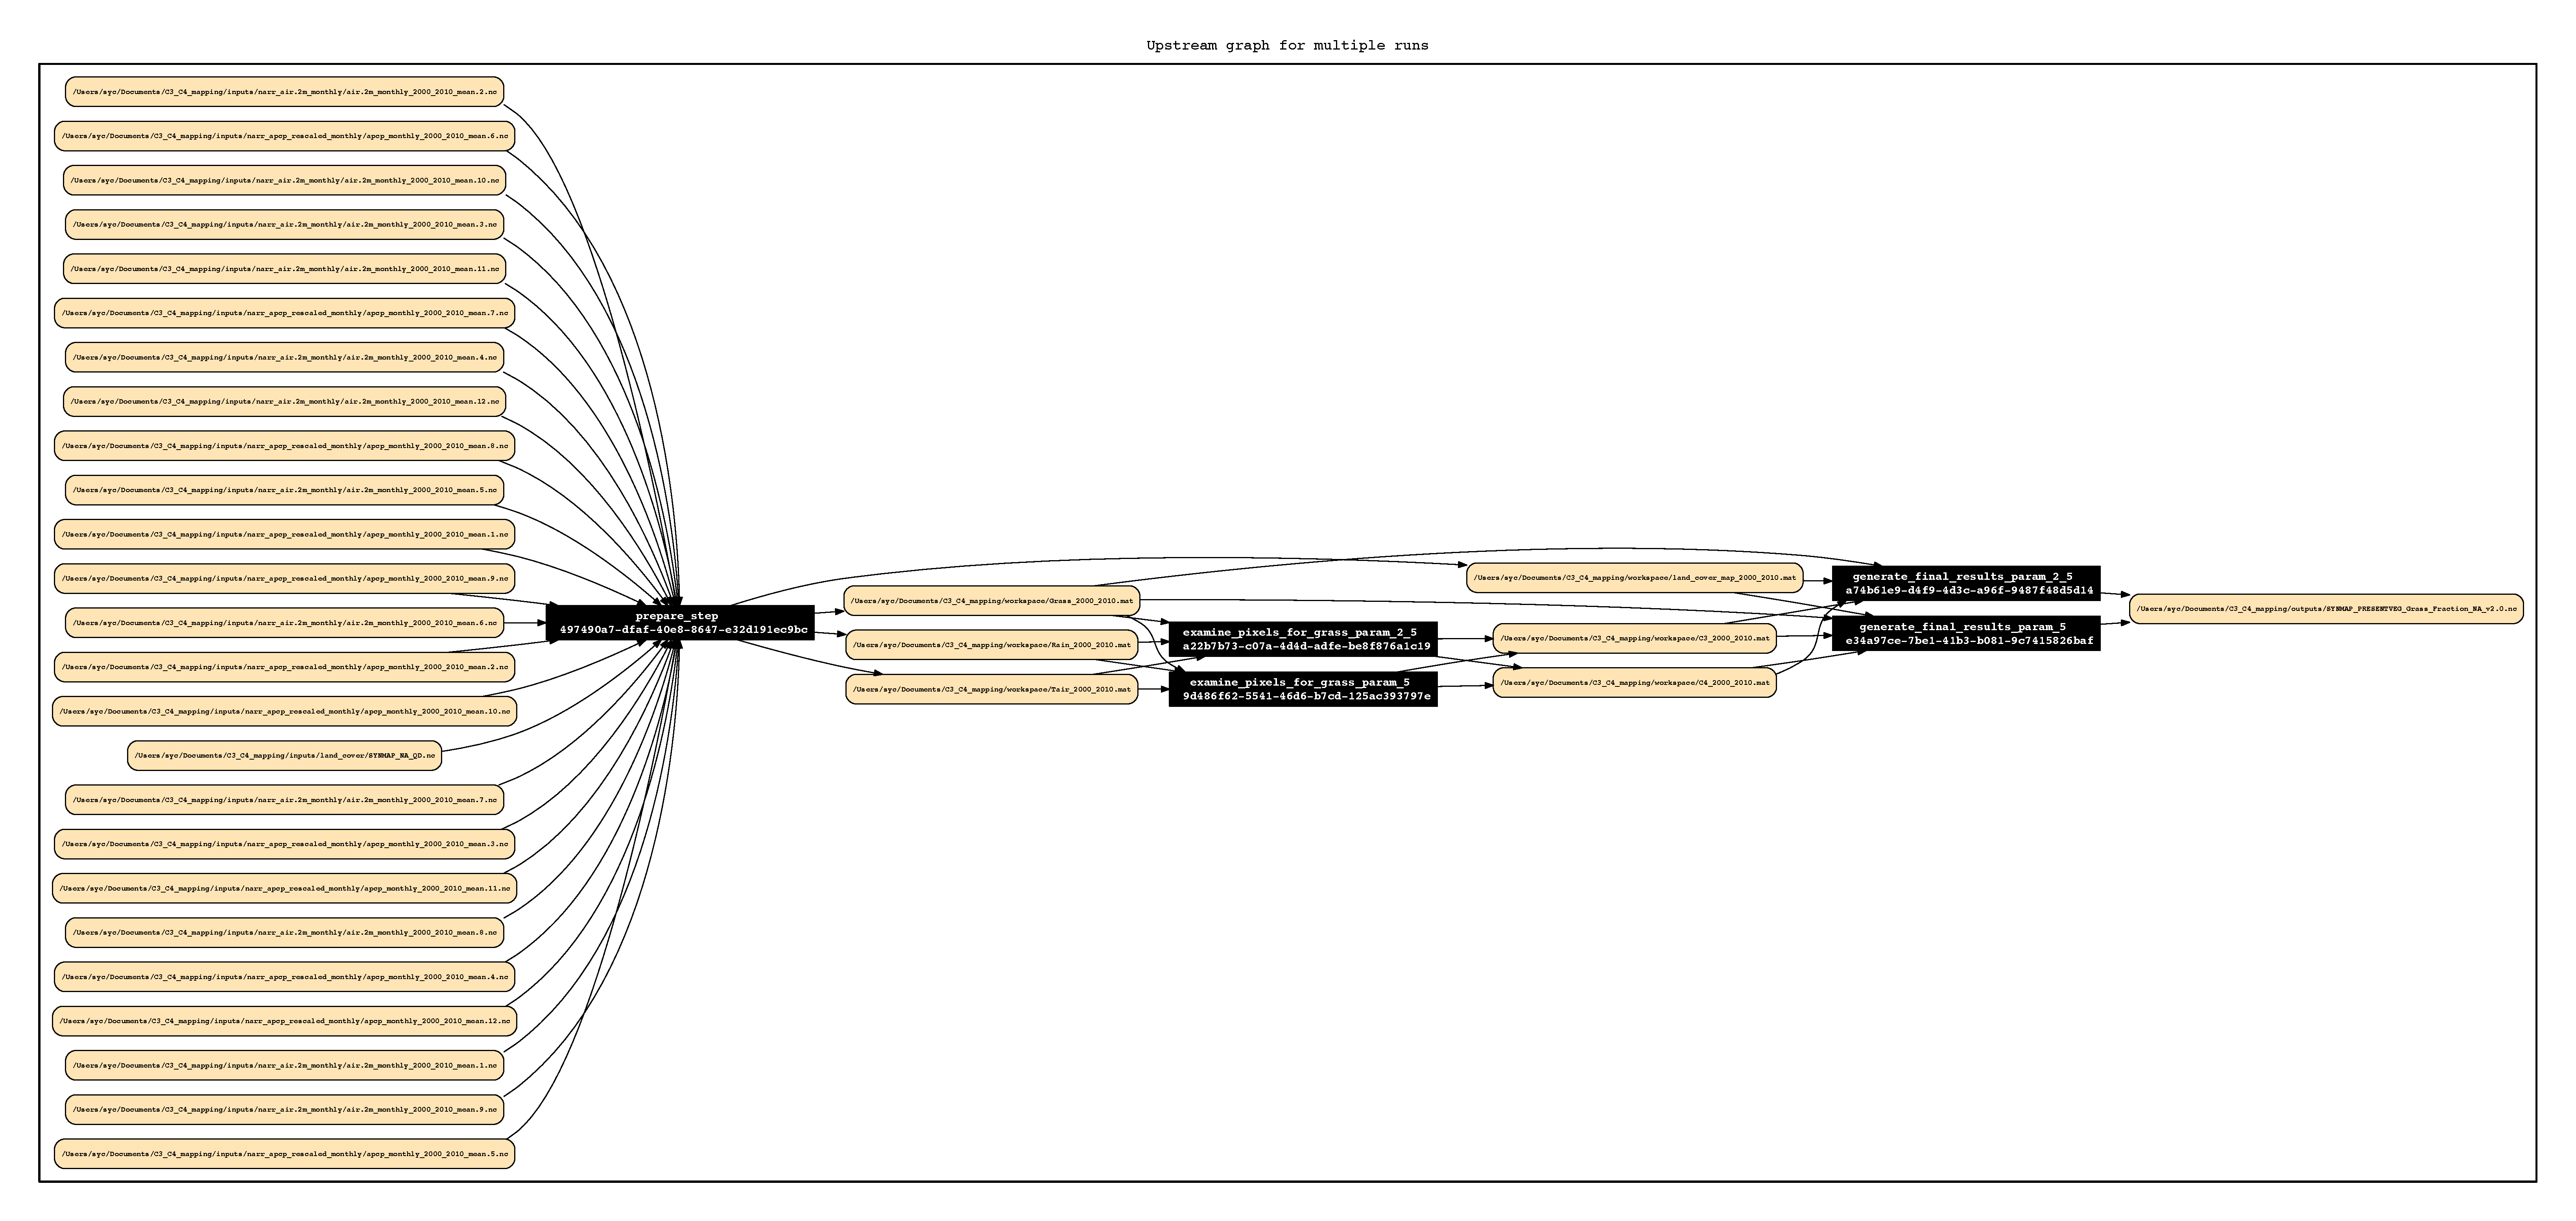
\includegraphics[height=4in, width=\columnwidth]{figures/C3C4v2_upstream_of_Grass_filePath} }} 
   \subfloat{{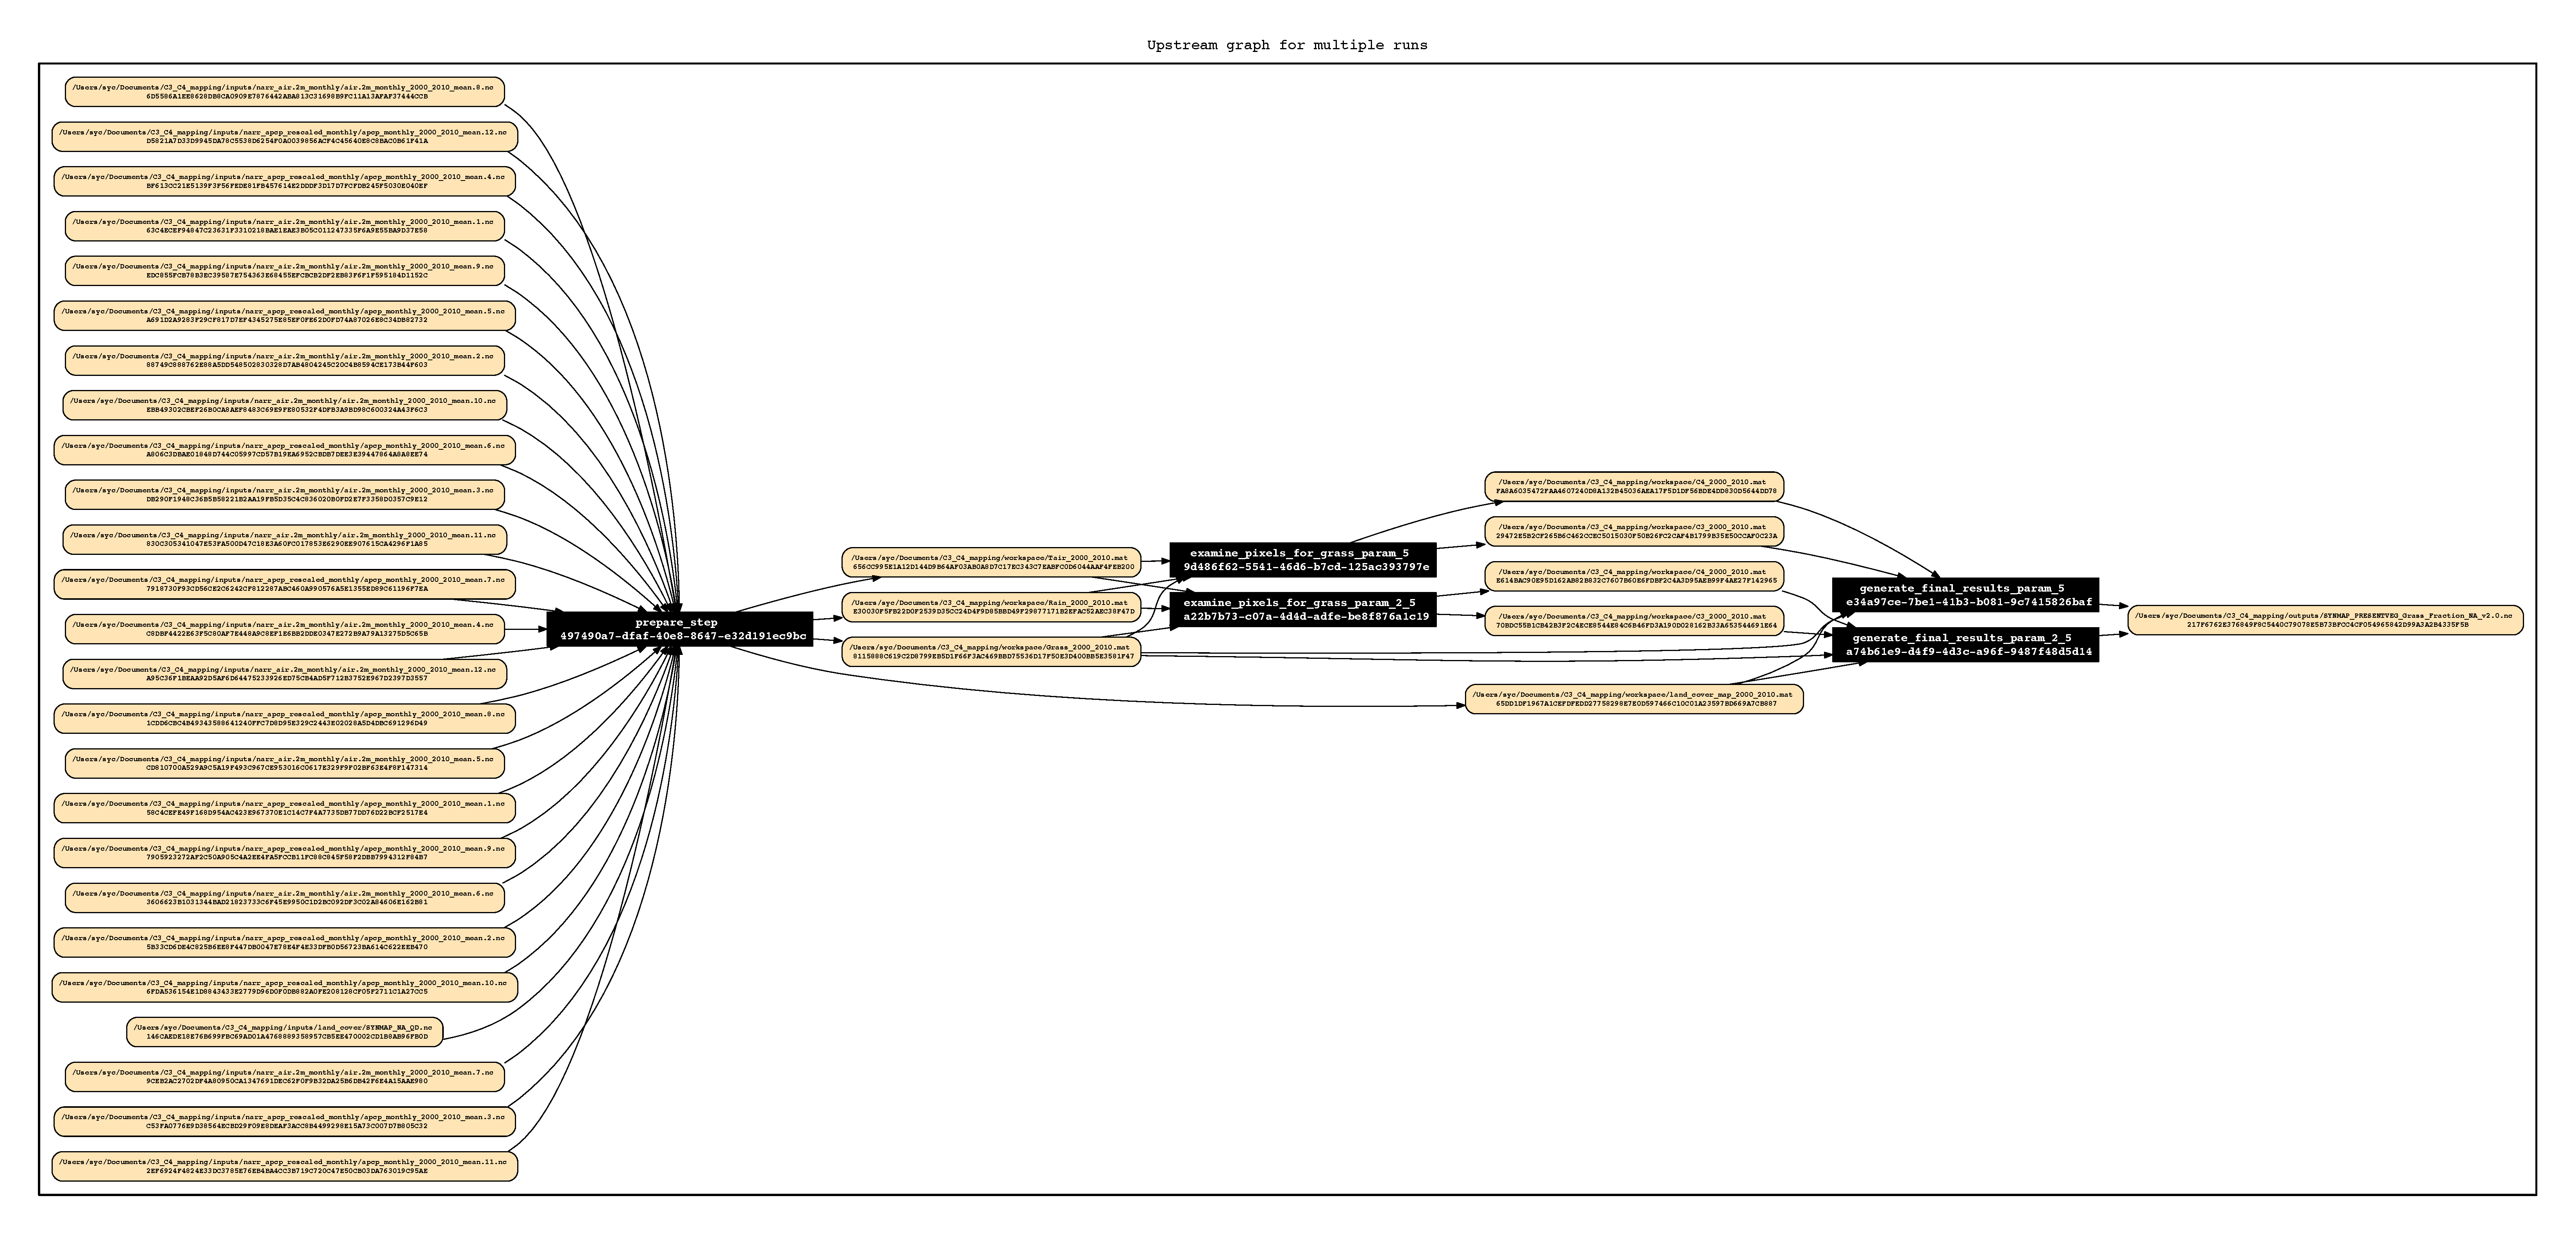
\includegraphics[height=4in, width=\columnwidth]{figures/C3C4v2_upstream_of_Grass_sha256} }}
   
  \caption{Upstream retrospective provenance subgraph (longitudinal view) that is relevant to one output ``\texttt{SYNMAP\_PRESENTVEG\_Grass\_Fraction\_NA\_v2.0.nc}" for C3C4 version 2 example. In the diagram, an orange yellow box represents a data file and a black box represents an execution (a run). }
  \label{fig:c3c4v2_filepath}
\end{figure}

\end{document}
